\mychapter{Literature}{Literature}{}\label{chap:literature}

\mysection{Dynamic Time Warping}{Dynamic Time Warping}\label{sec:dynamic-time-warping}
DTW is an algorithm for detecting the similarity of two signals, X and Y. This measure of similarity is achieved by calculating an optimal 
alignment cost between the two signals of length $N \in\mathbb{N}$  and $M \in\mathbb{N}$ respectively. In terms of feature vectors such as STFT or MFCC 
this means that each frame making up one signal is compared to each frame making up another signal. Using an alignment cost the best alignment for each 
frame in one to the other signal is chosen and an overall DTW cost is calculated to show how similar the overall signals are. The figure below shows that 
such an optimal alignment path may mean that a single frame in signal X may produce the lowest cost against more than one frame in signal Y.

\begin{figure}[H]
    \centering
    
\includegraphics[width=0.8\linewidth]{figures/background/vector_dtw.png}
    \caption{An example of the optimal warping path between two vector features, X with length N = 4 and Y with length M = 6}\label{fig:vector_dtw}
\end{figure}

The overall cost needed to determine how similar the two signals are is calculated via a cost matrix. Cost matrix, $C_{N+1, M+1}$ for signals X and Y, 
is initialised such that $C_{i, 0} = \infty$ for i = 1 to M, $C_{0, j} = \infty$ for j = 1 to M and $C_{0, 0} = 0$. 

The formula used to fill each cell of the cost matrix is:

\begin{equation}
C_{i, j} = \text{dist}(x_i, y_j) + \text{Q} \qquad \text{with} \quad \text{Q} = \min\begin{cases}
    C_{i-1, j-1} & \text{(match)} \\
    C_{i-1, j}   & \text{(insertion)} \\
    C_{i, j-1}   & \text{(deletion)}
\end{cases}
\end{equation}

$dist(x_i, y_j)$ represents the difference between $X_i$ and $Y_j$ as a distance. For vector signals this distance is calculated between each frame i 
of signal X and each fram j of signal Y. This can be done using various different techniques including cosine, euclidean or dot product similarity.
For this project only the cosine similarity and euclidean distance metrics were used.

Euclidean distance is sensitive to the magnitude and direction of the vectors for which it is calculated. In basic terms it is the absolute difference between 
two vectors.

\begin{equation}
    d(\mathbf{x_i}, \mathbf{y_j}) = \sqrt{(\mathbf{x_i}_1 - \mathbf{y_j}_1)^2 + (\mathbf{x_i}_2 - \mathbf{y_j}_2)^2 + \dots + (\mathbf{x_i}_n - \mathbf{y_j}_n)^2}
\end{equation}

Cosine similarity is only sensitive to the direction of the vectors for which it is calculated. In basic terms it is the angle between the two vectors.

\begin{equation}
    \cos(\mathbf{x_i}, \mathbf{y_j}) = \frac{\mathbf{x_i} \cdot \mathbf{y_j}}{\lVert\mathbf{x_i}\rVert \, \lVert\mathbf{y_j}\rVert}
\end{equation}

Q is the minimum value of three possible options namely match, insertion or deletion. Match is the value in the matrix cell diagonally down and left 
from the current cell for which the cost is being calculated. Insertion is the value in the matrix cell directly below the current cell and deletion is 
the matrix cell directly to the left of the current cell.

The cost which is then calculated for the current cell $C_{i, j}$ is a summation of the distance between the feature frames i and j in signals X and Y respectively 
as well as the lowest accumlated cost up until that point. This means that the final cell reached within the cost matrix, $C_{N+1, M+1}$ will contain the 
lowest overall cost for the similarity of signals X and Y. The lower the final cost, the higher the similarity between the two signals. The example shown in the 
figure is shown if X and Y are chosen to be scalar signals, however the same logic is used for when X and Y are vectors.

\begin{figure}[H]
    \centering
    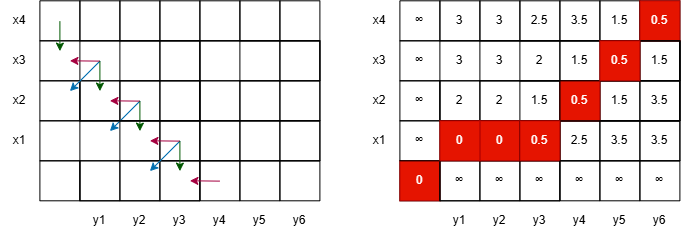
\includegraphics[width=0.8\linewidth]{figures/background/cost_matrix.png}
    \caption{An example for the three possible options for min as well as an example of the optimal warp path found for signals X and Y assuming X=[0, 2, 1, 0] 
    and Y=[0, 0, 0.5, 2, 1, 0]}\label{fig:cost_matrix}
\end{figure}

The general case of DTW finds global alignment between the two signals. This alignment is found using the warping path.

A $(N,M)$-warping path of length $L \in \mathbb{N}$ is
\begin{equation}
  P = (p_1, \ldots, p_L)
\end{equation}

with $p_\ell = (n_\ell, m_\ell) \in [1:N] \times [1:M]$ for $\ell \in [1:L]$ satisfying the following conditions:
\begin{itemize}
  \item Boundary condition: $p_1 = (1,1)$ and $p_L = (N,M)$
  \item Monotonicity condition: $n_1 \leq n_2 \leq \ldots \leq n_L$ and
        $m_1 \leq m_2 \leq \ldots \leq m_L$
  \item Step-size condition:
        $p_{\ell+1} - p_\ell \in \Sigma := \{(1,0), (0,1), (1,1)\}$
        for $\ell \in [1:L]$  % strictly this should be [1:L-1]
\end{itemize}

\mysection{Feature Extraction Methods}{Feature Extraction Methods}\label{sec:feature-extraction-methods-background}

\mysubsection{Short Time Fourier Transform}{Short Time Fourier Transform}\label{sec:short-time-fourier-transform}

\mysubsection{Mel-Frequency Cepstral Coefficients}{Mel-Frequency Cepstral Coefficients}\label{sec:mel-frequency-cepstral-coefficients}

\mysubsection{Linear Predictive Coding}{Linear Predictive Coding}\label{sec:linear-predictive-coding}